% ONLY IN CHAPTER 1

\addtocontents{toc}{\vspace{2em}} % Add a gap in the contents, for aesthetics


\pagestyle{fancy} 


\chapter{Introduction} 

\label{chap:ntroduction} 

\lhead{Chapter 1. \emph{Introduction}} 


In the field of discrete mathematics, the term ``graph" denotes a collection of distinct objects that may possess some form of pairwise connection or association. The discrete objects that make up the graph are referred to as nodes (or vertices), and their connections are known as edges (or arcs). This abstract structure can be employed to represent numerous real-world phenomena. For example, in an airline route map, nodes could symbolise airports, and edges could indicate the presence of a direct flight.

\vspace{0.1cm}

\begin{wrapfigure}{r}{0.42\linewidth}
	\centering
		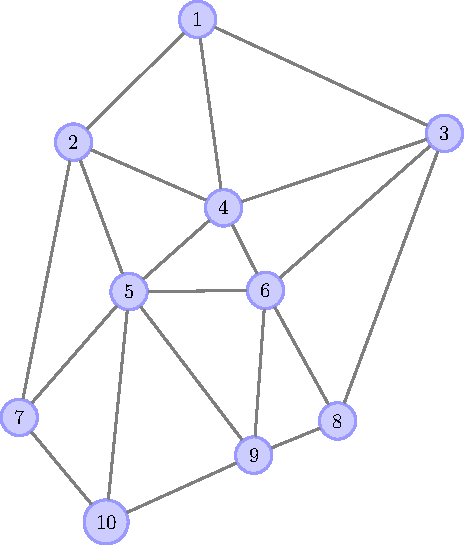
\includegraphics[width=0.9\linewidth]{Figures/graph_plot.pdf}
	\caption[A visual representation of a simple graph]{A visual representation of a simple graph with 10 nodes and 20 edges.}
	\label{fig:basic_graph}
\end{wrapfigure}


Graphs and network models are utilised in many actively researched areas of mathematics, including network processes such as epidemic modelling \citep{Pare2020}, Graph Neural Networks (GNNs) \citep{Zhou2020}, graphical models \citep{Holmes2008}, and semi-supervised learning \citep{Chong2020}.

\vspace{0.1cm}

In this thesis, the subject of focus is Graph Signal Processing (GSP), a rapidly evolving field that sits at the intersection of spectral graph theory, statistics, and data science \citep{Ortega2018}. GSP is an actively researched area devoted to the mathematical analysis of signals that are defined over the nodes of a graph, simply referred to as \textit{graph signals}. \phantom{In this thesis we are  }

\newpage

\begin{wrapfigure}{l}{0.4\linewidth}
	\centering
		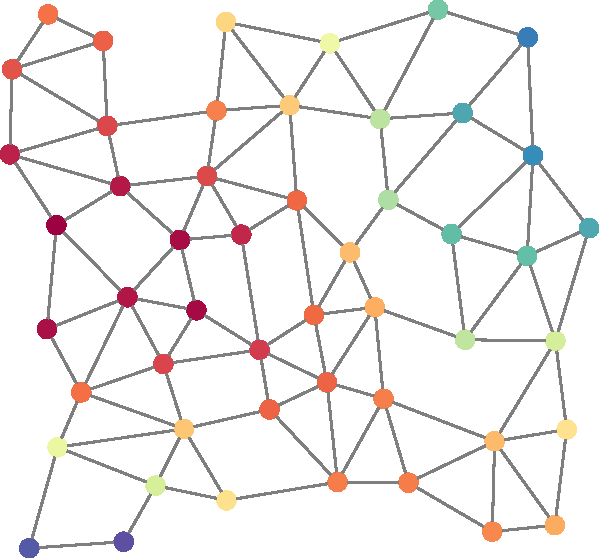
\includegraphics[width=0.95\linewidth]{Figures/graph_signal_plot.pdf}
	\caption[A graphical depiction of a graph signal]{A graphical depiction of a smooth graph signal. Here, the value of the signal at each node is represented by its colour.}
	\label{fig:graph_signal}
\end{wrapfigure}
 

A graph signal represents a value that is measured simultaneously at every node in a graph. For example, consider a social media network, where each node represents an individual, and the presence of an edge indicates that the two individuals have connected. An example of a graph signal in this context could be the age of each person in the network, or a score indicating their propensity to engage with certain content. In either case, this is a value that could theoretically be measured or estimated across the network, though it may be subject to missing data or noise. 

\phantom{In this thesis we are  }
\vspace{-0.3cm}

GSP typically uses tools that stem from classical signal processing, where the goal is to manipulate data that resides on a regular domain such as audio, images or radio. GSP utilises spectral graph theory to generalise these classical techniques, leading to graph-based counterparts of algorithms such as filtering, sampling, and reconstruction \citep{Shuman2013}. Applications of such methods are numerous, ranging from social networks \citep{Dong2015} and brain connectivity modelling \citep{Huang2018} to sensor networks \citep{Zhu2012}, and protein structures \citep{Srivastava2023}. GSP today remains rapidly evolving, with advancements in both theory and practical applications occurring constantly \citep{Leus2023}. As such, there are numerous opportunities for contribution, making it an exciting and dynamic area of research. 

\section{Research goals}

% multivariate

The goal of this thesis is to provide contributions to the areas of multivariate graph signal reconstruction and regression. A single signal, measured over a network comprising $N$ nodes, is an example of a univariate structure and can be described by a vector $\y \in \R^N$. Our methods, by contrast, are designed to be applicable to higher-dimensional objects. For example, $T$ samples of a graph signal measured across time can be described by a matrix $\Y \in \R^{N \times T}$. This kind of two-dimensional data can also be viewed as a single graph signal measured on the nodes of a Cartesian product graph \citep{Imrich2000}. More generally, a tensor-valued signal $\Yt \in \R^{N_1 \times N_2 \times ... \times N_d}$ can be understood as a signal on a $d$-dimensional Cartesian product graph \citep{Stanley2020}. 

% GSR + regression

Our aim is to expand the existing literature on multivariate GSP by presenting several novel Bayesian models for reconstructing partially observed graph signals, with and without additional explanatory variables. Graph signal reconstruction is a well-studied topic in GSP, however, the majority of published literature to date has focused on univariate, or time-varying signal models that provide point estimates for the missing values. We aim to generalise this in two ways. First, we present a rich Bayesian formulation, that outputs not only a point estimate but a full probability distribution quantifying prediction uncertainty. Furthermore, our goal is to produce models applicable to graph signals defined on arbitrary Cartesian product graphs, which naturally extend univariate and time-varying models. While the input to a graph signal reconstruction problem is typically only the partially observed graph signal and the topology of the underlying graph, we also consider the situation in which additional explanatory variables are available to aid in the estimation process. Therefore another key objective of ours is to produce graph signal regression models, applicable to a range of different data scenarios, that are robust to missing data. 

% sampling 

As mentioned, a key aspect of our models is the Bayesian formulation, which produces a full posterior probability distribution over the unknown reconstructed signal, rather than a single point estimate. Given the high-dimensional nature of the data, the posterior covariance, which contains information regarding the correlation between every element in the multivariate signal $\Yt$, is often too large to process with consumer-grade computer hardware. Therefore, another objective of ours is to develop efficient methods for extracting information regarding the prediction uncertainty. In particular, we consider two related but separate tasks: estimating the marginal posterior variance (node-level uncertainty) and drawing samples directly from the posterior. 

% binary

The majority of GSP models tend to focus on real-valued graph signals, leaving signals with binary or categorical entries relatively unexplored. It is therefore an additional goal of ours to develop new statistical reconstruction and regression algorithms for such graph signals. Although related tasks have been examined within semi-supervised learning in machine learning and GNNs in deep learning, we aim to introduce and showcase novel Bayesian models that are grounded firmly in the theoretical framework of GSP.

% complexity 

The high-dimensional nature of the models explored in this thesis comes with a unique set of challenges concerning computational robustness and efficiency. As such, a core objective is to reduce the computational cost of our algorithms wherever possible and to provide a detailed and transparent analysis of their time and memory complexity. The models we present are designed to be applicable to a wide range of application areas, and as such, throughout this thesis, we also provide illustrative examples and case studies to demonstrate their applicability. 

\newpage 


\section{GSP fundamentals}

\label{sec:fundamentals}

A graph, $\mathcal{G}$, with $N$ vertices is described by a node-set $\mathcal{V}$, and an edge set $\mathcal{E}$. In this thesis, we will be primarily concerned with undirected graphs without self-loops, meaning the edges have no preferential direction and nodes do not connect to themselves. By imposing some arbitrary but consistent ordering on the nodes, this graph can also be described by an $N \times N$ adjacency matrix $\A$, where the entry $\A_{ij} = \A_{ji} \geq 0$ holds the strength of connection between nodes $i$ and $j$. In the basic case of a non-weighted graph, $\A_{ij}$ is simply one if the corresponding edge exists and zero otherwise. Using the same ordering, a graph signal can be represented by a vector, $\y$, of length $N$, where $\y_i$ holds the value of the graph signal at node $i$. 

One key property of a graph signal is its \textit{smoothness}. Intuitively speaking, a smooth graph signal should exhibit gentle variation between closely connected nodes, as illustrated in \cref{fig:graph_signal}. Conversely, a rough graph signal might see large jumps in signal value between neighbouring nodes. Mathematically, the smoothness of a signal, $\y$, defined over the nodes of an undirected graph, can be measured in several ways. One simple option is the total square variation ($\text{TV}_2$), which is defined as follows. 

\begin{equation}
    \label{eq:TSV1}
    \text{TV}_2(\y) = \frac{1}{2}\sum_{i=1}^N \sum_{j=1}^N \A_{ij} (\y_i - \y_j)^2
\end{equation}

This metric, also known as Dirichlet energy, sums up the square difference in signal value at each neighbouring node, weighted by the corresponding entry in the adjacency matrix, with the factor of a half adjusting for the double counting of nodes. It can also be written in terms of a single quadratic form, by introducing a new matrix $\LL$ - the so-called graph \textit{Laplacian}. 

\begin{equation}
    \label{eq:TSV2}
    \text{TV}_2(\y) = \y^\top \LL \y
\end{equation}

The Laplacian, like the adjacency matrix $\A$, is another symmetric $N \times N$ matrix and is defined as $\LL = \D - \A$, where $\D$ is the degree matrix. $\D$ is a diagonal operator, where entry $\D_{ii}$ holds the sum of all the edge weights linked to node $i$, or in other words, the vector along the diagonal of $\D$ is the column (or row) sum of $\A$. The Laplacian, which can be interpreted as a generalisation of the discrete second-order derivative operator for an irregular topology, is of central importance to many aspects of GSP \citep{Shuman2013}. 

\newpage

It is straightforward to show that the two expressions for the total square variation given in \cref{eq:TSV1,eq:TSV2} are equivalent; see for example chapter 3 of \cite{Ortega2022}. A few basic facts stand out about the Laplacian quadratic form.

\begin{enumerate}
    \item $\y^\top \LL \y \geq 0$ for any $\y$. Since $\text{TV}_2(\y)$ sums the square difference between the signal at each pair of nodes, weighted by the non-negative entries of the adjacency matrix, the Laplacian quadratic form must be strictly non-negative. By definition, this implies that the matrix $\LL$ is positive semi-definite (PSD). 
    \item $\one^\top \LL \one = 0$, where $\one$ is a length-$N$ vector of ones. If the signal of interest is constant over the whole graph, the total square variation must be zero. Moreover, if the graph contains two or more isolated sub-graphs, with edges connecting nodes within each clique but not between cliques, then any signal that is constant over each sub-graph will have a total square variation of zero. 
\end{enumerate}

Since $\LL$ is positive semi-definite, its eigenvalues are all real and non-negative, and its eigenvectors can be chosen to be real and orthonormal. Thus, $\LL$ can be decomposed as follows. 

\begin{equation}
    \LL = \U \LAM \U^\top
\end{equation}

Here, $\U$ is the orthogonal, $N \times N$ matrix of eigenvectors $\{\uu_i\}$, and $\LAM$ is the diagonal matrix of corresponding eigenvalues $\{\lambda_i\}$, typically arranged in ascending order. As $\U$ is orthonormal, it holds that $\uu_i^\top \uu_j = \delta_{ij}$, and that $\{\uu_i\}$ form a set spanning $\R^N$. Given the definition of the Laplacian quadratic form, the eigenvectors are the unique set of orthonormal vectors that sequentially minimise the total square variation, subject to perpendicularity to all those preceding \citep{Spielman2019}.


$$
\begin{matrix}
    \uu_1 & = & \underset{\raisebox{-0.1cm} { $ \scriptstyle |\uu|^2 = 1$ }}{\text{argmin}} \quad & \text{TV}_2(\uu) \\[0.7cm]
    \uu_2 & = & \underset{\raisebox{-0.1cm} { $ \scriptstyle |\uu|^2 = 1, \; \perp \uu_1$ }}{\text{argmin}} \quad & \text{TV}_2(\uu) \\[0.7cm]
    \uu_3 & = & \underset{\raisebox{-0.1cm} { $ \scriptstyle |\uu|^2 = 1, \;\perp \uu_1, \uu_2$ }}{\text{argmin}} \quad & \text{TV}_2(\uu) \\[0.7cm]
    \uu_4 & = & \ldots
\end{matrix}
$$

\newpage

In this way, the eigenvectors of the graph Laplacian can be understood as sequentially less smooth with respect to the topology of the graph. The corresponding eigenvalue, referred to as the frequency, gives a value specifying how ``rough'' each eigenvector is relative to the others, as measured by $\text{TV}_2$. Note that, for any undirected graph, the first Laplacian eigenvector will always be constant with an eigenvalue of zero. \Cref{fig:uk_eigs} gives a visual depiction of the first eight Laplacian eigenvectors and eigenvalues for a network representing local authority regions in the UK. \footnote{Using boundary data published by the Office for National Statistics \citep{ONS2019}}  

\begin{figure}[t]
	\centering
		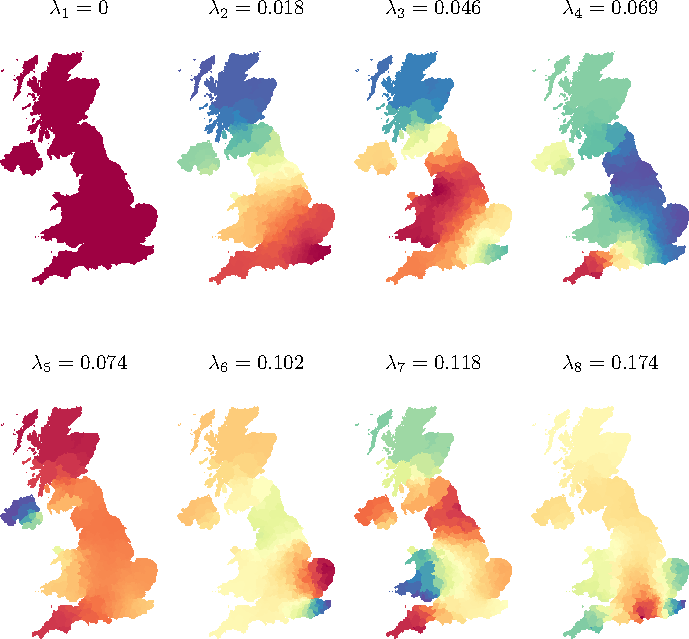
\includegraphics[width=0.85\linewidth]{Figures/uk_plot.pdf}
		% \rule{35em}{0.5pt}
        \caption[A visualisation of the Laplacian eigenvectors for a network of regions in the UK]{A visualisation of the first eight Laplacian eigenvectors, alongside their associated eigenvalues, for a network of local authority regions in the UK. Each node represents a region, and each pair of regions share an edge if they border one another (or have a direct ferry crossing). Colour is used to represent the value of the graph signal at each node.  }
	\label{fig:uk_eigs}
\end{figure}


Since $\{\uu_i\}$ span the total space of $\R^N$, any graph signal, $\y$, can be decomposed into a weighted sum of the Laplacian eigenvectors. This parallels the classical Fourier transform, which expands signals into the basis of complex exponentials \citep{Sneddon1995}. As such, any graph signal, $\y$, has a dual representation, $\z$, in the frequency domain. Transformations between these two representations can be achieved by applying the Graph Fourier Transform (GFT) and Inverse Graph Fourier Transform (IGFT), which amount to multiplying by the matrices $\U^\top$ and $\U$, respectively.

\begin{align}
    \z &= \mkern 2mu \text{GFT}(\y) \mkern 2mu = \U^\top \y \\[0.2cm]
    \y &= \text{IGFT}(\z)  = \U \z
\end{align}

For some simple graphs, the GFT is equivalent to a well-known transform in classical signal processing. For example, the Laplacian of the cycle graph (i.e. a set of nodes connected in a loop) has eigenvectors that can be expressed as sines and cosines (or, in full generality, complex exponentials) as visualised in \cref{fig:cycle_eighs}. This concept has been used to establish a rigorous connection between GSP and classical signal processing, through the study of Algebraic Signal Processing (ASP) \citep{Puschel2003, Sandryhaila2013}. With the GFT and IGFT defined, a wide range of potential models is opened up, many of which can be understood as direct generalisations of methods from conventional signal processing. Classical tasks such as filtering, denoising, reconstruction, sampling, compression etc. can all be translated into the GSP paradigm, setting the stage for a new era of signal processing that leverages graph structures for more complex and rich data analysis, and opening the door to a wealth of novel applications.

\begin{figure}[t]
	\centering
		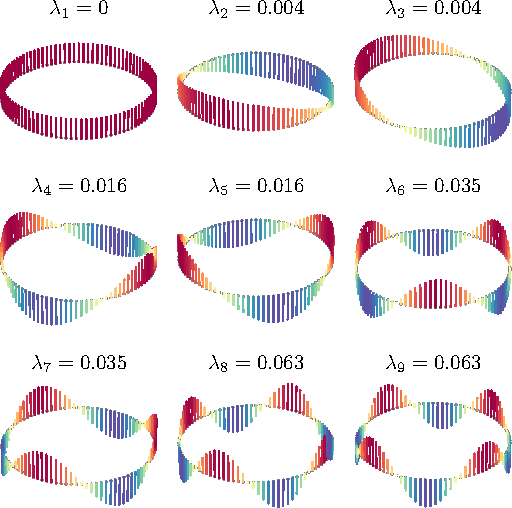
\includegraphics[width=0.65\linewidth]{Figures/loop_plot.pdf}
        \caption[A visualisation of the Laplacian eigenvectors of the cycle graph]{A visualisation of the first nine Laplacian eigenvectors of a cycle graph with 50 nodes, along with their associated eigenvalue.}
	\label{fig:cycle_eighs}
\end{figure}


\newpage

\section{Example applications}

Graph signal processing methods have proven effective in numerous real-world applications. In this brief section, we highlight several use cases from the literature to serve as motivation for the content of this thesis. Many of these areas are used as illustrative examples for the methods developed in this work.


\subsection{Biology}

The world of biology provides numerous interesting use cases for graph signal processing methods \citep{Li2023}. One area which has garnered significant interest is in analysing protein-protein interactions. Here, the concept is to model a set of proteins as nodes in an ``interactome'', which is the network of physical molecular interactions in a particular cell. Recent work such as \cite{Colonnese2021} used GSP methods to predict new interactions between proteins, while work such as \cite{Jha2022} used graph neural networks for the same task. These models aim to automate the prediction of protein interactions, reducing the time and cost associated with experimental methods. Other work has modelled an individual protein molecule as a network of residues connected based on their physical distance in 3D space, to predict its biophysical properties \citep{Srivastava2023}. 

Another domain in biology that has benefited from GSP methods is brain connectivity modelling. Studies such as \cite{Goldsberry2017, Atasoy2016, Menoret2017, Itani2021} have found that the graph-spectral frequency profile of signals derived from fMRI imaging can provide valuable insight into brain activity. Specifically, these and related works have identified specific Laplacian spectral profiles associated with different emotional states, task familiarity, and neurological diseases.

\subsection{Transportation and infrastructure}

Another domain in which GSP methods have been extensively applied is transportation and infrastructure. In \cite{Hasanzadeh2017}, the authors propose an adaptive ARMA model in the graph frequency domain for real-time traffic prediction, achieving a substantial performance increase over non-graph-aware alternatives. Traffic prediction was also addressed using GSP methods in \cite{Chakraborty2017} with a technique known as trend filtering \citep{Wang2016}. Automatic incident detection using spatiotemporally denoised thresholds was applied in \cite{Chakraborty2019}. In \cite{Xiu2022}, the authors used a spatial-temporal multi-graph convolutional wavelet network to predict passenger numbers on a metro system.

GSP has also been employed to analyse patterns of power consumption in electricity grids \citep{Ramakrishna2021}, pressure in hydraulic networks \citep{Zhou2022} and leak detection in water networks \citep{Orn2022}. In \cite{He2018} and \cite{Zheng2022}, the authors utilised GSP to address non-intrusive load disaggregation—an active area of research in the field of smart grids and energy conservation where the goal is to estimate each appliance's contribution to total consumption. In \cite{Ying2022}, the authors tackle the recovery of harmonic data lost during power transmission, based on spectral graph theory, and in \cite{Wang2022b}, the authors use GSP to identify abnormal batteries from cell-level voltage signals in a network of electric bicycle charging stations.


\subsection{Finance and economics}

Networks have been used in financial and economic models for many years \citep{Marti2021}, yet recently GSP has found some interesting use cases. In \cite{Vinicius2020}, the authors employ a spectral model to learn an underlying graph structure from financial time-series data, showing that meaningful physical interpretations related to the market index factor can be extracted from this representation. In \cite{Zhang2023}, the authors consider how GSP can be incorporated into momentum-based financial forecasting models, demonstrating that the additional topological information can enhance the accuracy of such models.

GSP has also been used recently in the context of asset allocation and portfolio theory. The portfolio cut paradigm, introduced in \cite{Dees2020}, is a graph-theoretic portfolio partitioning technique that enables investors to group economically meaningful clusters of assets. In \cite{Arroyo2022}, this concept is extended to include a dynamic portfolio, with time-evolving clusters.

Graph Neural Networks have also been used extensively in financial applications \citep{Wang2022c}. 


\subsection{Sensor networks}

Sensor networks are a classic application for GSP methods, as a graph is typically straightforward to construct from the physical positioning of the devices \citep{Jablonski2017}. Many applications in this domain focus on distributed algorithms, as sensors and IoT devices are naturally suited to local communication. The aims of such applications are varied, encompassing tasks like compression \citep{Zhu2012}, denoising \citep{Tay2021}, reconstruction \citep{Wang2015}, and distributed data processing \citep{Chi2022}.

Some of the earliest work classified as GSP involved applications with sensor data, for example, \cite{Guestrin2004}. Here, the authors used local basis functions to design a regression algorithm capable of fast convergence with only local communication. In \cite{Wagner2005}, the authors develop a distributed wavelet transform and applied it to a signal compression task over a network of sensors. 


\section{Contributions}

In this thesis, we present several contributions to the theory and practice of graph signal processing, the most prominent of which are summarised below. 

\begin{itemize}
    \item We propose a parametrised family of low-pass filters for signals on Cartesian product graphs composed of two or more factor graphs. 
    \item Using these filters to construct graph-spectral priors, we propose a holistic Bayesian framework for reconstruction and regression tasks with partially observed, real-valued signals on Cartesian product graphs. 
    \item We give practical advice for implementing such models by providing a detailed analysis of their runtime complexity as a function of the model hyperparameters and input data composition. 
    \item We present PyKronecker, a Python library for the efficient and scalable manipulation of Kronecker-structured operators and tensor-valued signals. 
    \item We propose and evaluate several methods for characterising the posterior covariance of our models that are scalable to large graphs with multiple tensor dimensions. 
    \item We extend and generalise our reconstruction and regression algorithms to graph signals that contain binary or categorical observations. 
\end{itemize}


\section{Thesis organisation}

The core content of this thesis begins in \cref{chap:gsr_2d}, with the reconstruction of signals on general two-dimensional Cartesian product graphs. Here, we introduce our Bayesian model formulation and present two iterative algorithms for computing the posterior mean. In \cref{chap:kgr_rnc_2d}, we consider how the reconstruction problem can be modified by introducing additional explanatory variables, leading to three novel multivariate regression models applicable to different modelling scenarios. In \cref{chap:nd_gsp}, we generalise the reconstruction and regression techniques developed in the preceding two chapters to $d$-dimensional tensor-valued data, under the ``Multiway" GSP (MWGSP) framework. This is followed, in \cref{chap:variance}, by an investigation into the posterior covariance of the models, where we develop scalable techniques for estimating the marginal variance and direct sampling. Finally, in \cref{chap:binary}, we modify the reconstruction and regression algorithms to handle binary and categorical graph signals. Along the way, there are several methodological contributions as well as some detailed case studies. We begin, in \cref{chap:lit_review}, by defining the precise scope of this thesis, reviewing the relevant literature, and presenting a more detailed breakdown of our core contributions. 
